%%
%% ACM CCS 2026 submission — sigconf format
%% Double-blind: all author information MUST be commented out
%%
\documentclass[sigconf,anonymous]{acmart} %% CCS: DO NOT REMOVE

\AtBeginDocument{%
  \providecommand\BibTeX{{Bib\TeX}}}

%% Rights management — SAMPLE values, DO NOT REMOVE
\setcopyright{acmlicensed}
\copyrightyear{2026}
\acmYear{2026}
\acmDOI{XXXXXXX.XXXXXXX}
\acmConference[CCS '26]{Proceedings of the 2026 ACM SIGSAC Conference on Computer and Communications Security}{November 15--19, 2026}{The Hague, The Netherlands}
\acmISBN{978-1-4503-XXXX-X/2026/11}

%% Additional packages (acmart includes most standard ones)
\usepackage{booktabs}
\usepackage{multirow}
\usepackage{enumitem}
\usepackage[capitalise,nameinlink]{cleveref}

%% TikZ / PGF for diagrams
\usepackage{tikz}
\usetikzlibrary{arrows.meta, positioning, shapes.geometric, fit, calc, backgrounds, decorations.pathreplacing}
\usepackage{pgfplots}
\pgfplotsset{compat=1.18}

\begin{document}

\title{Online Context-Aware LLM Man-in-the-Middle Attacks on Cyber-Physical Systems}

%% CCS: Authors MUST be commented out for double-blind submission
% \author{Anonymous}
% \affiliation{%
%   \institution{Anonymous Institution}
%   \country{Anonymous}}
% \email{anonymous@example.com}

\renewcommand{\shortauthors}{Anonymous}

\begin{abstract}
We present \textbf{CPSForge}, a framework that places an LLM as a man-in-the-middle agent in live PLC communication, automating both red team (attack injection) and blue team (anomaly blocking) on the real-time tag stream. The same model, context pipeline, and decision loop serve both roles---differing only in the prompt. Every 1.5\,s the agent observes the PLC state via S7 protocol, reasons about the process phase, and decides to attack or wait (red team) or allow or block a proposed write (blue team). A mandatory safety shield mediates every write.

We evaluate CPSForge on three industrial scenes connected to a real Siemens S7-1200 PLC across \textbf{333 runs} spanning six research questions: context ablation, fine-tuning, online-vs-static attack modes, seven defense configurations, cross-model robustness (1.7B--3B), and frontier model scaling (GPT-4o-mini). Key findings: (1)~the online MITM achieves up to 54\% ASR with a 3B local model and 100\% with GPT-4o-mini, while a static one-shot LLM generates zero valid proposals; (2)~the LLM defender blocks 100\% of attacks---including cross-model blocking of frontier-model proposals---but with 98.7\% false-positive rate (block-everything policy); (3)~the ``self-deterrence'' effect observed under rich context with 3B models vanishes at frontier scale; and (4)~QLoRA fine-tuning on verified PLC traces improves attack success from 0\% to 37\% while preserving defense capability. To the best of our knowledge, CPSForge is the first framework to deploy an LLM as a live MITM for closed-loop CPS red/blue team analysis on real PLC hardware.
\end{abstract}


%%
%% CCS concepts — generate at http://dl.acm.org/ccs.cfm
%%
\begin{CCSXML}
<ccs2012>
 <concept>
  <concept_id>10002978.10002991.10002992</concept_id>
  <concept_desc>Security and privacy~Intrusion detection systems</concept_desc>
  <concept_significance>500</concept_significance>
 </concept>
 <concept>
  <concept_id>10002978.10003014</concept_id>
  <concept_desc>Security and privacy~Systems security</concept_desc>
  <concept_significance>500</concept_significance>
 </concept>
 <concept>
  <concept_id>10010520.10010553.10010562</concept_id>
  <concept_desc>Computer systems organization~Embedded and cyber-physical systems</concept_desc>
  <concept_significance>300</concept_significance>
 </concept>
</ccs2012>
\end{CCSXML}

\ccsdesc[500]{Security and privacy~Intrusion detection systems}
\ccsdesc[500]{Security and privacy~Systems security}
\ccsdesc[300]{Computer systems organization~Embedded and cyber-physical systems}

\keywords{cyber-physical systems, industrial control systems, large language models, man-in-the-middle attacks, PLC security, red teaming, runtime defense}

\maketitle

\section{Introduction}
\label{sec:intro}

Industrial PLCs exchange actuator commands, sensor readings, and setpoints with connected machines over field protocols (Siemens S7, Modbus, OPC-UA) every few milliseconds. An adversary with protocol-level network access can read this stream, infer the process state, and inject writes timed to cause physical damage---overflowing a tank, missorting products, or disabling safety interlocks. Conversely, a defender observing the same stream can detect writes inconsistent with the controller's current behavior and block them before execution.

Recent work has applied LLMs to CPS security: AttackLLM~\cite{ahmed2025attackllm} generates process-aware attacks offline on static traces; MALF~\cite{ning2025malf} fuzzes industrial protocols at the packet layer; PentestGPT~\cite{deng2024pentestgpt} and Hackphyr~\cite{rigaki2024hackphyr} automate IT penetration testing. HARVEY~\cite{garcia2017harvey} demonstrated closed-loop PLC MitM with a hand-crafted physics model. None embed an LLM in a live PLC control loop as both attacker and defender.

\textbf{Insight.} The live PLC tag stream carries exactly the information needed for both attack and defense reasoning. By placing an LLM as a man-in-the-middle in this stream---reading the same tags an attacker or defender would observe---we can automate both roles symmetrically. The same model, observation pipeline, and context structure serve as red team and blue team, differing only in the prompt.

\textbf{CPSForge} is a framework that places an LLM as a man-in-the-middle agent in real PLC communication. Every 1.5\,s, it reads the tag stream via S7 protocol, assembles a context prompt from observed data, and queries the LLM: as red team, \emph{attack} or \emph{wait}; as blue team, \emph{allow} or \emph{block}. A mandatory safety shield mediates every write. The framework is configuration-driven: any PLC-connected plant requires only a scene YAML---no code changes.

We evaluate CPSForge on three Factory~I/O scenes connected to a real Siemens S7-1200 PLC across \textbf{333 runs} organized into six research questions (context ablation, fine-tuning, online-vs-static modes, defense configurations, cross-model robustness, frontier model scaling). Our contributions are:

\begin{itemize}[leftmargin=1.2em,nosep]
    \item \textbf{C1.~Online LLM MITM for CPS red/blue teaming.} A closed-loop LLM agent that operates inside the PLC control loop: observe $\to$ infer phase $\to$ build context $\to$ decide (attack$|$wait) $\to$ act $\to$ observe result. Unlike AttackLLM (offline), MALF (packet-level), or HARVEY (hand-crafted physics model), CPSForge uses general-purpose LLM reasoning with a configuration-driven scene abstraction. The same architecture serves as an LLM blue team agent, creating a symmetric attacker--defender pairing.

    \item \textbf{C2.~Context-ablation study.} Three strictly controlled context tiers---minimal (tag values only), partial (+ history + descriptions), full (+ phase inference + action effects)---measure the minimum adversary knowledge required for effective CPS attacks. We discover a ``self-deterrence'' effect: rich context suppresses 3B-class model attacks but \emph{not} frontier-scale models.

    \item \textbf{C3.~Dual-objective fine-tuning.} QLoRA training on 2{,}057 examples (verified attacks + defense decisions) improves red team ASR from 0\% to 37\% on a continuous-control scene while preserving 100\% blue team blocking---testing whether attack-aware training transfers to defense.

    \item \textbf{C4.~Defense comparison.} Seven defense configurations---rule-based (threshold, phase-aware, intent-consistency), LLM-only, and combined---enable the first systematic comparison of runtime defense types against LLM-generated CPS attacks.

    \item \textbf{C5.~Multi-scale model evaluation.} Cross-model comparison from 1.7B (Qwen3) through 3B (Qwen2.5, SmolLM3) to frontier-scale (GPT-4o-mini), demonstrating that attack capability and self-deterrence are model-scale-dependent, and that a local 3B defender generalizes to block frontier-model attacks.
\end{itemize}

The rest of the paper is organized as follows: \S\ref{sec:background} provides background; \S\ref{sec:threat} defines the threat model; \S\ref{sec:design} presents the architecture; \S\ref{sec:methodology} describes the evaluation methodology; \S\ref{sec:evaluation} presents results; \S\ref{sec:discussion} discusses findings and limitations; \S\ref{sec:related} reviews related work; \S\ref{sec:conclusion} concludes.

\section{Background and Motivation}
\label{sec:background}

\subsection{CPS Communication and Attack Surface}

Industrial PLCs execute control logic at 1--10\,ms scan cycles, reading sensors, computing outputs, and updating actuators on every cycle. Communication with SCADA/HMI systems occurs over field protocols (S7, Modbus, OPC-UA) that expose process data blocks containing all tag values. On many deployed systems---including the Siemens S7-1200 in default configuration---these data blocks are readable and writable by any network-reachable host without authentication.

This creates a well-documented attack surface: an adversary with S7-level access can read the live tag stream (sensor values, actuator states, setpoints) and inject writes at the process-semantic level. Real-world CPS attacks from Stuxnet~\cite{langner2011stuxnet} to PIPEDREAM~\cite{cisa2022pipedream} exploited exactly this---manipulating process data within existing protocols rather than deploying novel exploits. Stuxnet wrote to PLC data blocks~\cite{falliere2011w32}; Industroyer issued standard IEC~60870-5-104 commands~\cite{cherepanov2017industroyer}; the Oldsmar attacker changed a single setpoint~\cite{cisa2021oldsmar}. The trend is toward reusable, protocol-aware attack frameworks: PIPEDREAM provides modular OT-specific tools targeting multiple PLC families~\cite{greenberg2022pipedream}.

\subsection{LLMs for CPS Security: State and Gap}

LLMs have been applied to CPS security in several ways: AttackLLM~\cite{ahmed2025attackllm} generates process-aware attacks on static traces; LLM4PLC~\cite{fakih2024llm4plc} synthesizes PLC invariants; LLM-based IDS approaches~\cite{ann2024ids_llm,sharshar2025explainable} classify historical traffic logs. In the adjacent domain of autonomous cyber agents, PentestGPT~\cite{deng2024pentestgpt} and Hackphyr~\cite{rigaki2024hackphyr} automate IT penetration testing, and MALF~\cite{ning2025malf} fuzzes industrial protocols at the packet layer.

However, none of these approaches embed an LLM in a \emph{live} PLC control loop---observing real tag values, reasoning about the process phase in real time, and executing writes whose physical consequences are immediately observable. Without closed-loop execution it remains unclear whether LLM-generated strategies survive practical constraints (timing, process physics, controller overwrite), and whether defenses improve meaningfully after exposure to such attacks.

\subsection{PLC-in-the-Loop Evaluation}

CPSForge addresses this gap by combining a real Siemens S7-1200 PLC with Factory~I/O, a software-based process emulator. Every tag value the LLM observes is a real S7 protocol read; every write is a real S7 write that changes the controller's data block. Unlike offline evaluations, the LLM sees what a real adversary would see: live tag values updating every 500\,ms, with real controller dynamics. This \emph{PLC-in-the-loop} design is essential for studying online-vs-static attack modes (RQ3), LLM defense under real timing (RQ4), and whether rich context changes model behavior on live systems (RQ1).
\section{Threat Model}
\label{sec:threat}

\subsection{Adversary Model}

CPSForge models a \emph{post-compromise adversary} with S7 protocol-level network access to the PLC---achieved, e.g., through credential theft, insider access, or lateral movement from the IT network. This is realistic: S7 communication is commonly exposed on flat industrial networks, and tools such as python-snap7 allow any network-reachable host to read and write PLC data blocks without authentication on many deployed configurations.

\textbf{Capabilities.} The adversary can: (i)~continuously read the live tag stream (sensor values, actuator states, setpoints) at polling rate; (ii)~infer the current operational phase from tag patterns; (iii)~inject writes to writable tags in the PLC data block. Attacks are expressed at the \emph{process-semantic level}---actuator overrides, setpoint shifts, sensor spoofing, timing delays, and sequence perturbations---not firmware or memory-level modifications. The exact attack surface is scene-specific (Table~\ref{tab:attack_surface}).

\textbf{Goals.} Cause measurable physical impact (unsafe state transitions, degraded performance, incorrect sequencing) while remaining process-valid. When possible, maintain plausible sensor/actuator patterns to delay detection.

\subsection{LLM Agent Role}

The LLM operates as a man-in-the-middle in the tag stream, not as a trusted controller. Every three polling cycles (1.5\,s), it receives a structured snapshot of the observed tags and returns a structured decision: as red team, \emph{attack} or \emph{wait} (with a complete write specification); as blue team, \emph{allow} or \emph{block} (with suspicion score). All outputs are treated as untrusted proposals. The safety shield enforces tag whitelists, value ranges, duration caps, and process invariants before any write reaches the PLC.

\textbf{Timing.} LLM inference takes 13--33\,s per call (3B model, depending on context tier). This positions the adversary as a \emph{supervisory-timescale} attacker making strategic interventions at multi-second intervals---consistent with documented ICS incidents, where Stuxnet operated over weeks~\cite{langner2011stuxnet}, Ukraine grid attacks over minutes~\cite{liang2017ukraine}, and even HARVEY~\cite{garcia2017harvey} operated at 100\,ms--1\,s. The 10-attack budget tests whether the LLM can \emph{select the right writes} from limited opportunities.

\subsection{Attack Surface}
\label{sec:threat:attack_surface}

Table~\ref{tab:attack_surface} enumerates the concrete variables accessible via S7 protocol across our three evaluation scenes. All reside in non-optimized PLC data blocks readable/writable by python-snap7 without authentication. The ``PLC refresh'' column indicates whether the PLC overwrites the variable each scan cycle ($\checkmark$) or trusts the stored value ($\times$)---a critical distinction for attack persistence.

\begin{table}[t]
\centering
\caption{LLM-accessible attack surface per scene.}
\label{tab:attack_surface}
\small
\begin{tabular}{@{}llllc@{}}
\toprule
\textbf{Scene} & \textbf{Variable} & \textbf{Type} & \textbf{Category} & \textbf{Refresh} \\
\midrule
\multirow{4}{*}{\shortstack[l]{Level\\Control}} & SetpointIn & REAL & Setpoint hijack & $\times$ \\
& FillValve & REAL & Actuator override & $\checkmark$ \\
& DischargeValve & REAL & Actuator override & $\checkmark$ \\
& Enable & BOOL & Safety kill & $\times$ \\
\midrule
\multirow{5}{*}{\shortstack[l]{Sorting\\Weight}} & LightThresh & REAL & Threshold manip. & $\times$ \\
& HeavyThresh & REAL & Threshold manip. & $\times$ \\
& iState & INT & State jump & $\checkmark$ \\
& Conveyor1/2/3 & BOOL & Actuator override & $\checkmark$ \\
& Sorter1/2 & BOOL & Actuator override & $\checkmark$ \\
\midrule
\multirow{5}{*}{\shortstack[l]{Sorting\\Height}} & iState & INT & State jump & $\checkmark$ \\
& TurnTimer & INT & Timer accel. & $\checkmark$ \\
& DwellTimer & INT & Timer accel. & $\checkmark$ \\
& Enable & BOOL & Safety kill & $\times$ \\
& IsTall & BOOL & Flag spoof & $\checkmark$ \\
\bottomrule
\end{tabular}
\end{table}

\subsection{Defender Model}

The defender observes the same tag stream plus experiment telemetry. Depending on configuration, it uses static thresholds, process invariants, phase-aware rules, intent-consistency checks, or LLM-based anomaly detection (\S\ref{sec:design}). The defender has no oracle knowledge of attacker intent; logged attacks can be used for offline adaptation.

\subsection{Scope}

This evaluation focuses on I/O-level data manipulation---the attacker reads/writes PLC I/O tags via standard S7 protocol. Written values to PLC-refreshed tags are overwritten each scan cycle, requiring precise timing or continuous injection. The safety shield bounds all writes to process-safe ranges, so reported attack success rates reflect effectiveness within this configured envelope. The framework does not model firmware compromise, PLC root access, or unrestricted code deployment.

\section{System Design}
\label{sec:design}

CPSForge is a closed-loop LLM red/blue team framework for CPS security analysis. It comprises five interacting layers---physical execution, observation, red team (attack generation), safety enforcement, and blue team (defense)---connected to a real PLC. The same LLM serves both roles with different prompts. The framework is configuration-driven: any PLC-connected plant can be analyzed by providing a scene YAML. Figure~\ref{fig:architecture} illustrates the pipeline.

\begin{figure*}[t]
    \centering
    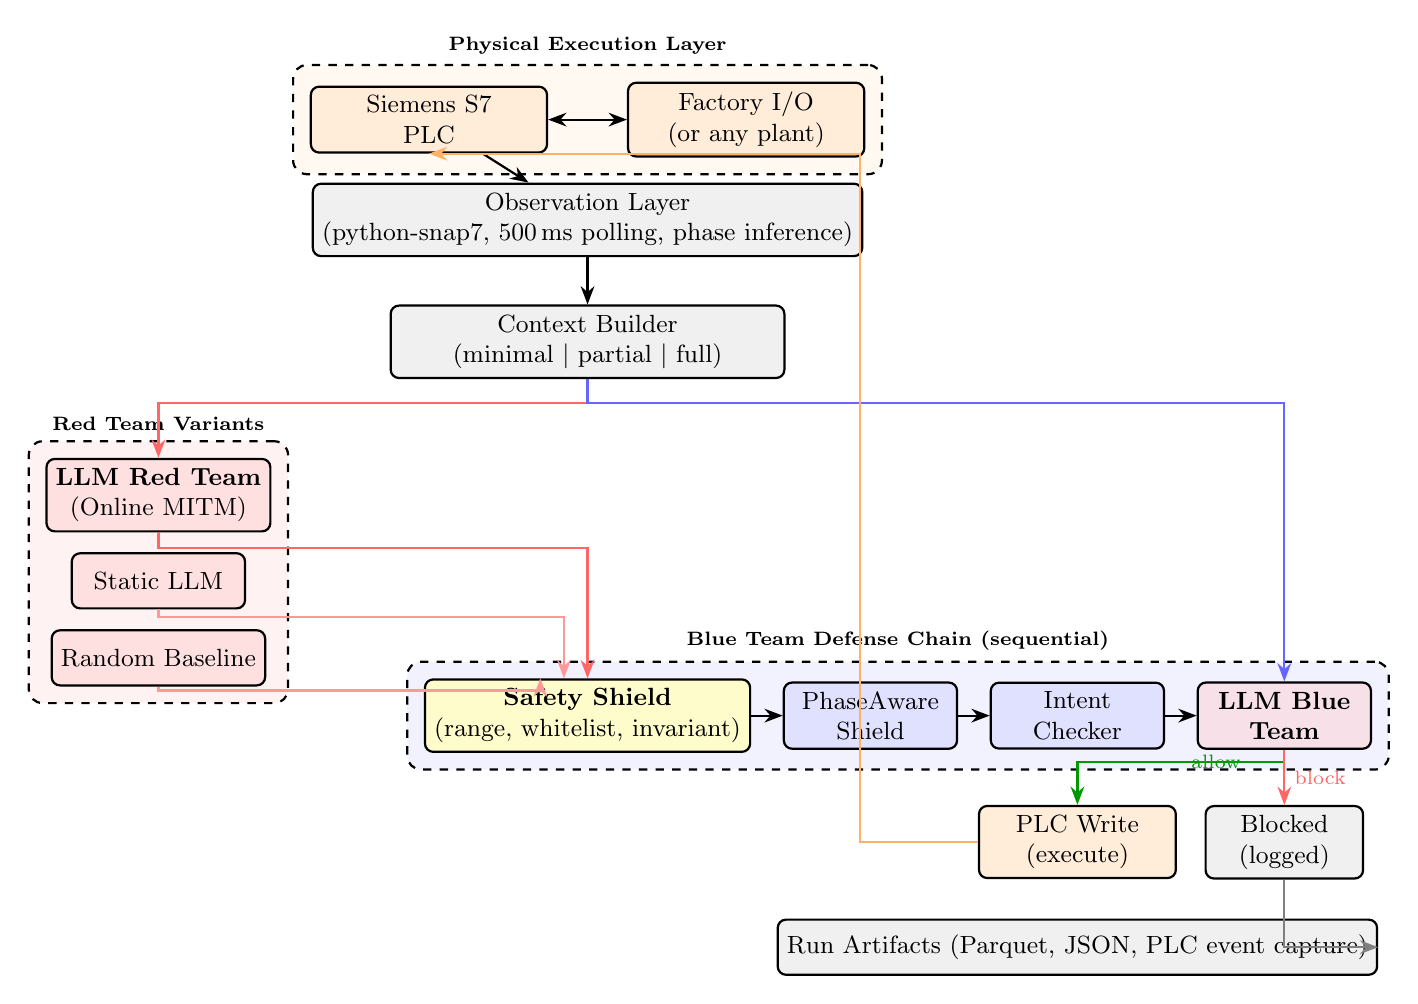
\begin{tikzpicture}[
        >=Stealth,
        node distance=0.6cm and 0.5cm,
        every node/.style={font=\small},
        layer/.style={draw, rounded corners=3pt, minimum width=2.2cm, minimum height=0.7cm, align=center, thick},
        plcbox/.style={layer, fill=orange!15, minimum width=3cm},
        atkbox/.style={layer, fill=red!12},
        shieldbox/.style={layer, fill=yellow!20},
        defbox/.style={layer, fill=blue!12},
        logbox/.style={layer, fill=gray!12},
        llmbox/.style={layer, fill=purple!12},
        groupbox/.style={draw, dashed, rounded corners=5pt, inner sep=6pt, thick},
        arr/.style={->, thick, >=Stealth},
        darr/.style={<->, thick, >=Stealth},
    ]

    %% ===== Physical Execution Layer =====
    \node[plcbox] (plc) {Siemens S7\\PLC};
    \node[plcbox, right=1.0cm of plc] (fio) {Factory I/O\\(or any plant)};
    \draw[darr] (plc) -- (fio);

    %% ===== Observation Layer =====
    \node[logbox, below=0.8cm of $(plc)!0.5!(fio)$, minimum width=5.0cm] (mw) {Observation Layer\\(python-snap7, 500\,ms polling, phase inference)};
    \draw[arr] (plc) -- (mw);

    %% ===== Context Builder =====
    \node[logbox, below=0.6cm of mw, minimum width=5.0cm] (ctx) {Context Builder\\(minimal $|$ partial $|$ full)};
    \draw[arr] (mw) -- (ctx);

    %% ===== Red Team (left) =====
    \node[atkbox, below left=1.0cm and 1.5cm of ctx, minimum width=2.5cm] (llm_atk) {\textbf{LLM Red Team}\\(Online MITM)};
    \node[atkbox, below=0.25cm of llm_atk] (static_atk) {Static LLM};
    \node[atkbox, below=0.25cm of static_atk] (random_atk) {Random Baseline};

    %% Context to red team
    \draw[arr, red!60] (ctx.south) -- ++(0,-0.3) -| (llm_atk.north);

    %% ===== Defense Chain (center-right) — sequential =====
    \node[shieldbox, below=3.8cm of ctx, minimum width=3.0cm, minimum height=0.7cm] (shield) {\textbf{Safety Shield}\\(range, whitelist, invariant)};

    \node[defbox, right=0.4cm of shield, minimum width=2.2cm] (phase_shield) {PhaseAware\\Shield};
    \node[defbox, right=0.4cm of phase_shield, minimum width=2.2cm] (intent) {Intent\\Checker};
    \node[llmbox, right=0.4cm of intent, minimum width=2.2cm] (llm_def) {\textbf{LLM Blue}\\
    \textbf{Team}};

    %% Red team proposals → defense chain (sequential)
    \draw[arr, red!60] (llm_atk.south) -- ++(0,-0.2) -| (shield.north);
    \draw[arr, red!40] (static_atk.south) -- ++(0,-0.1) -| ([xshift=-0.3cm]shield.north);
    \draw[arr, red!40] (random_atk.south) -- ++(0,-0.05) -| ([xshift=-0.6cm]shield.north);

    %% Sequential defense chain arrows
    \draw[arr] (shield) -- (phase_shield);
    \draw[arr] (phase_shield) -- (intent);
    \draw[arr] (intent) -- (llm_def);

    %% Context to blue team LLM
    \draw[arr, blue!60] (ctx.south) -- ++(0,-0.3) -| (llm_def.north);

    %% ===== PLC Write or Block =====
    \node[plcbox, below=0.7cm of intent, minimum width=2.5cm] (write) {PLC Write\\(execute)};
    \node[logbox, below=0.7cm of llm_def, minimum width=2.0cm] (block) {Blocked\\(logged)};
    \draw[arr, green!60!black] (llm_def.south) -- ++(0,-0.15) -| (write.north) node[pos=0.25, right, font=\scriptsize]{allow};
    \draw[arr, red!60] (llm_def.south) -- (block) node[midway, right, font=\scriptsize]{block};

    %% Arrow back to PLC
    \draw[arr, thick, orange!60] (write.west) -- ++(-1.5,0) |- (plc.south);

    %% ===== Artifacts =====
    \node[logbox, below=0.5cm of write, minimum width=4.5cm] (artifacts) {Run Artifacts (Parquet, JSON, PLC event capture)};
    \draw[arr, gray] (block.south) |- (artifacts.east);

    %% ===== Group boxes =====
    \begin{scope}[on background layer]
        \node[groupbox, fill=orange!5, fit=(plc)(fio), label={[font=\scriptsize\bfseries]above:Physical Execution Layer}] {};
        \node[groupbox, fill=red!5, fit=(llm_atk)(static_atk)(random_atk), label={[font=\scriptsize\bfseries]above:Red Team Variants}] {};
        \node[groupbox, fill=blue!5, fit=(shield)(phase_shield)(intent)(llm_def), label={[font=\scriptsize\bfseries]above:Blue Team Defense Chain (sequential)}] {};
    \end{scope}

    \end{tikzpicture}
    \caption{CPSForge architecture. The observation layer polls the real PLC and builds context for both red and blue team LLMs. Attack proposals flow through the sequential defense chain: Safety Shield $\to$ PhaseAwareShield $\to$ IntentChecker $\to$ LLM Blue Team. A write must pass all stages to reach the PLC. The same model and context pipeline serve both roles.}
    \label{fig:architecture}
\end{figure*}

\subsection{Physical Execution Layer}

A Siemens S7-1200 PLC executes control logic deployed from TIA Portal~v17. Factory~I/O serves as the process emulator. Communication uses python-snap7 over Ethernet at 500\,ms polling. Each scene is defined by a YAML profile containing tag metadata (addresses, types, ranges), process descriptions, attack surface definitions, safety rules, and reset procedures. Three scenes cover continuous and discrete processes:

\begin{itemize}[leftmargin=1.2em,nosep]
    \item \textbf{Level Control} (15~tags): continuous PID tank fill/drain.
    \item \textbf{Sorting by Weight} (35~tags): discrete 3-way weight classification.
    \item \textbf{Sorting by Height} (30~tags): discrete 2-way height sorting.
\end{itemize}

\subsection{Observation and Context Layer}
\label{sec:design:context}

The middleware reads PLC tags every 500\,ms, constructing structured snapshots (sensor values, actuator states, setpoints, alarms, derived features). A rule-based phase inference engine determines the current operational phase from snapshot patterns. A modular context builder assembles three tiers for the RQ1 ablation:

\begin{itemize}[leftmargin=1.2em,nosep]
    \item \textbf{Minimal:} current tag values only. No history, descriptions, or ranges.
    \item \textbf{Partial:} values + 5-step history + tag descriptions + short scene summary + derived features (rates of change, moving averages).
    \item \textbf{Full:} values + 10-step history + inferred phase + prior action effects + attack guidance + safety rules.
\end{itemize}

The same context builder serves both red and blue team LLMs, ensuring a fair information basis.

\subsection{LLM Attacker Layer}
\label{sec:design:attacker}

Three attacker variants enable controlled comparison (RQ3):

\paragraph{Random Baseline.} Bounded random perturbations over the scene's attack surface. Provides the lower bound.

\paragraph{Static LLM.} One-shot batch: receives scene context and a single snapshot, proposes attacks without process feedback.

\paragraph{Online MITM (C1).} The core contribution. Every $k{=}3$ polling cycles: (1)~observe current PLC state; (2)~inspect history; (3)~infer phase; (4)~assemble context-tier prompt; (5)~LLM decides attack or wait; (6)~if attack, emit structured JSON with target tag, value, duration, reasoning; (7)~pass through defense chain; (8)~observe result; (9)~continue iteratively.

All LLM outputs must parse into a strict \texttt{AttackDecision} JSON schema. Invalid outputs default to ``wait.'' Attack budget: max 10 per run. The LLM never receives raw PLC addresses---only symbolic tag names.

\subsection{Safety Shield}
\label{sec:design:shield}

The mandatory first gate before any write reaches the PLC. It evaluates sequential checks: (1)~whitelist (tag must be in declared attack surface); (2)~range (value within configured bounds); (3)~duration cap; (4)~cooldown window; (5)~mutual exclusion (conflicting actuators cannot be simultaneously active); (6)~invariant (hard physical-boundary rules). The shield runs in microseconds and is always active regardless of defense variant. It also generates a rollback plan (original values for automatic restoration after attack expiry).

\subsection{Defense Layer}
\label{sec:design:defense}

Seven defense configurations (RQ4) organized into three categories:

\paragraph{Baseline.} Threshold and invariant detectors (rule-based).

\paragraph{Novel Rule-Based Defenses.} \emph{PhaseAwareShield}: blocks writes inconsistent with the current operational phase (e.g., opening discharge during fill). Standard range checks cannot catch contextually wrong but individually legal values. \emph{IntentConsistencyChecker}: blocks writes opposing the controller's current trend (e.g., forcing fill valve open while PID is reducing it).

\paragraph{LLM Defender (C4).} Uses the \emph{same model, context builder, and inference pipeline} as the attacker, with a defense-oriented prompt. For each proposed write that passes the safety shield, it receives: current process state, proposed write details, scene description, inferred phase. It outputs: \texttt{\{decision: allow|block, suspicion\_score: 0--1, reasoning\}}. On parse failure, defaults to ``allow'' to avoid blocking legitimate writes. This creates a symmetric LLM-vs-LLM evaluation.

The full defense chain applies sequentially: Safety Shield $\to$ PhaseAwareShield $\to$ IntentChecker $\to$ LLM Defender $\to$ Execute. Each stage can independently block a write.

\subsection{Fine-Tuning Pipeline}
\label{sec:design:finetune}

QLoRA fine-tuning (C3) trains Qwen2.5-3B-Instruct on 2{,}057 examples: 83~post-hoc verified successful attack traces (tag moved toward injected value), 608~defense ``block'' examples (known attack proposals), and 1{,}366~defense ``allow'' examples (normal operation with synthetic legitimate writes). Configuration: rank=16, $\alpha$=32, dropout=0.05, 3~epochs, lr=$2{\times}10^{-4}$, 4-bit NF4 quantization. Trainable parameters: 29.9M (0.96\% of 3.1B).

\section{Evaluation Methodology}
\label{sec:methodology}

\subsection{Experiment Matrix}

We organize 333 live PLC runs into six research questions:

\begin{description}[leftmargin=1.2em,nosep,style=nextline]
    \item[RQ1 (Context):] How does context depth affect LLM attack capability?
    \item[RQ2 (Fine-tuning):] Does QLoRA fine-tuning change attack and defense capability?
    \item[RQ3 (Attack mode):] Does online feedback outperform one-shot attack?
    \item[RQ4 (Defense):] Which defense configurations block LLM attacks?
    \item[RQ5 (Cross-model):] Are trends robust across model architectures?
    \item[RQ6 (Frontier):] Does GPT-4o-mini differ qualitatively from local 3B models?
\end{description}

\noindent Table~\ref{tab:matrix} summarizes the experiment matrix.

\begin{table}[t]
\centering
\caption{Experiment matrix (333 runs total).}
\label{tab:matrix}
\small
\begin{tabular}{@{}lrc@{}}
\toprule
\textbf{RQ} & \textbf{Runs} & \textbf{Variables} \\
\midrule
RQ1 Context     & 27  & 3 ctx $\times$ 3 scenes $\times$ 3 rep \\
RQ2 Fine-tune   & 36  & 2 models $\times$ 2 ctx $\times$ 3 scenes $\times$ 3 rep \\
RQ3 Attack mode & 27  & 3 attackers $\times$ 3 scenes $\times$ 3 rep \\
RQ4 Defense     & 126 & 2 models $\times$ 7 defs $\times$ 3 scenes $\times$ 3 rep \\
RQ5 Cross-model & 72  & 3 models $\times$ 2 ctx $\times$ 2 atk $\times$ 2 scenes $\times$ 3 rep \\
RQ6 Frontier    & 45  & 3 ctx + 2 defs $\times$ 3 scenes $\times$ 3 rep \\
\bottomrule
\end{tabular}
\end{table}

Each run: 60 steps at 500\,ms polling; the LLM is called every 3 steps; attack budget of 10 per run; wall-clock time 6--10 min (local) or 2--5 min (API). Hardware: Siemens S7-1200 PLC, Dell Precision 5820 with RTX A4000 16\,GB, Windows~11.

\subsection{Models}

\textbf{Primary:} Qwen2.5-3B-Instruct (4-bit NF4), base and QLoRA-finetuned.
\textbf{Cross-model (RQ5):} Qwen3-1.7B, SmolLM3-3B (all 4-bit NF4).
\textbf{Frontier (RQ6):} GPT-4o-mini via OpenAI API; local Qwen2.5-3B serves as defender.

\subsection{Metrics}

\textbf{ASR} $= N_{\text{succ}}/N_{\text{exec}}$: post-hoc success, comparing tag value at step $N{-}1$ vs.\ $N{+}2$ (success if tag moved toward injected value).
\textbf{VAR} $= N_{\text{valid}}/N_{\text{submitted}}$: schema-valid JSON output rate.
\textbf{Prevention rate} $= N_{\text{blocked}}/N_{\text{proposals}}$.

\textbf{Statistical note.} With 3 repeats per cell, we report Wilson 95\% CIs. The design detects large effects ($\Delta$ASR $>$ 30\,pp) and zero-vs-nonzero differences, but cannot reliably distinguish moderate effects ($\approx$10\,pp) from noise.

\section{Evaluation}
\label{sec:evaluation}

All results are from live PLC runs. ASR values are lower bounds under the safety shield: an unconstrained adversary could achieve higher ASR. This constraint applies uniformly and does not affect within-table comparisons.

\subsection{RQ1: Context Ablation}
\label{sec:eval:rq1}

Table~\ref{tab:context_ablation} shows how context depth affects attack capability (Qwen2.5-3B, no defense).

% Table 3 --- RQ1 Context Ablation
% Generated by: python -m cpsforge.analysis.generate_tables
% RQ-specific filtering: limited to 3 runs per (scene, context) cell
\begin{table}[t]
\centering
\caption{RQ1: Context ablation for online MITM attacker (base Qwen2.5-3B; no RQ4 defense active; safety shield always active).}
\label{tab:context_ablation}
\small
\setlength{\tabcolsep}{3pt}
\begin{tabular}{llrrrrrr}
\toprule
\textbf{Scene} & \textbf{Context} & \textbf{Runs} & \textbf{Prop.} & \textbf{Writes} & \textbf{Succ.} & \textbf{ASR\%} & \textbf{Lat.(ms)} \\
\midrule
Level Control & Minimal & 3 & 23 & 2 & 0 & 0.0 & 13086 \\
 & Partial & 3 & 20 & 13 & 0 & 0.0 & 18429 \\
 & Full & 3 & 5 & 0 & 0 & 0.0 & 7863 \\
\midrule
Sort.~Weight & Minimal & 3 & 13 & 13 & 7 & 53.8 & 17929 \\
 & Partial & 3 & 12 & 5 & 2 & 40.0 & 19789 \\
 & Full & 3 & 0 & 0 & 0 & 0.0 & 11180 \\
\midrule
Sort.~Height & Minimal & 3 & 30 & 30 & 1 & 3.3 & 16906 \\
 & Partial & 3 & 30 & 25 & 1 & 4.0 & 22944 \\
 & Full & 3 & 30 & 30 & 4 & 13.3 & 22263 \\
\bottomrule
\end{tabular}
\vspace{2pt}
\noindent\footnotesize{3 repeats per configuration; ASR computed post-hoc.}
\end{table}

\textbf{Finding 1: Self-deterrence under rich context.} Full context produces \emph{zero} attack proposals on Sorting by Weight---the model decides ``wait'' on every call across all repeats. On Level Control, full context reduces proposals from 23 (minimal) to 5, all shield-blocked. Rich operational context (phase inference, safety rules) makes the 3B model overly cautious.

\textbf{Finding 2: Self-deterrence is scene-dependent.} On Sorting by Height, full context is the \emph{most} effective tier (13.3\% ASR vs.\ 3.3\% at minimal)---the discrete state-machine logic benefits from richer phase context. On Sorting by Weight, partial context achieves 40\% ASR while full drops to zero proposals.

\textbf{Finding 3: Context changes strategy.} Minimal context produces brute-force overrides. Partial shifts toward setpoint manipulation. Full, when it does attack (Sort.~Height), targets a narrow set of tags with deliberate overrides. More context makes the model more selective but also more conservative.

\textbf{Implication:} Exposing operational context may itself serve as a defense---deterrence through transparency.

\subsection{RQ2: Fine-Tuning Impact}
\label{sec:eval:rq2}

Table~\ref{tab:finetune_comparison} compares base vs.\ QLoRA-finetuned Qwen2.5-3B.

% Table RQ2 --- Fine-Tuning Comparison
% Generated by: python -m cpsforge.analysis.generate_tables
% RQ-specific filtering: limited to 3 runs per (scene, context, model) cell
\begin{table}[t]
\centering
\caption{RQ2: Fine-tuning effect on attack capability (online MITM, no defense). Base = Qwen2.5-3B-Instruct; FT = same model with QLoRA v2 adapter. VAR = schema-valid outputs / LLM calls.}
\label{tab:finetune_comparison}
\small
\setlength{\tabcolsep}{3pt}
\resizebox{\columnwidth}{!}{%
\begin{tabular}{lllrrrrrrr}
\toprule
\textbf{Scene} & \textbf{Ctx} & \textbf{Model} & \textbf{Runs} & \textbf{LLM calls} & \textbf{VAR\%} & \textbf{Prop.} & \textbf{Writes} & \textbf{Succ.} & \textbf{ASR\%} \\
\midrule
Level Control & Minimal & Base & 3 & 27 & 100.0 & 23 & 2 & 0 & 0.0 \\
 & Minimal & FT & 3 & 30 & 100.0 & 30 & 30 & 11 & 36.7 \\
 & Full & Base & 3 & 15 & 100.0 & 5 & 0 & 0 & 0.0 \\
 & Full & FT & 3 & 34 & 0.0 & 0 & 0 & 0 & 0.0 \\
\midrule
Sort.~Weight & Minimal & Base & 3 & 14 & 92.9 & 13 & 13 & 7 & 53.8 \\
 & Minimal & FT & 3 & 30 & 100.0 & 30 & 16 & 0 & 0.0 \\
 & Full & Base & 3 & 5 & 40.0 & 0 & 0 & 0 & 0.0 \\
 & Full & FT & 3 & 60 & 0.0 & 0 & 0 & 0 & 0.0 \\
\midrule
Sort.~Height & Minimal & Base & 3 & 30 & 100.0 & 30 & 30 & 1 & 3.3 \\
 & Minimal & FT & 3 & 30 & 100.0 & 30 & 30 & 3 & 10.0 \\
 & Full & Base & 3 & 30 & 100.0 & 30 & 30 & 4 & 13.3 \\
 & Full & FT & 3 & 45 & 0.0 & 0 & 0 & 0 & 0.0 \\
\bottomrule
\end{tabular}%
}
\vspace{2pt}
\noindent\footnotesize{3 repeats per configuration; ASR computed post-hoc.}
\end{table}

\textbf{Finding 4: Fine-tuning enables attacks on Level Control.} The finetuned model achieves 36.7\% ASR (11/30 writes) on Level Control minimal, vs.\ 0\% for the base model. Training teaches the model to propose shield-legal values.

\textbf{Finding 5: Schema regression under full context.} The finetuned model achieves VAR=0\% under full context on all scenes---every output fails schema validation. This is a prompt-length distributional mismatch: training examples come from shorter prompts; full-context prompts ($\sim$1.5--2K tokens) fall outside the training distribution. Addressable by augmenting training data with full-context examples.

\textbf{Finding 6: Defense capability preserved.} The finetuned LLM defender retains 100\% blocking on Sort.~Height (Table~\ref{tab:defense_finetuned}), confirming dual-role training preserves defense while modifying attack behavior.

\subsection{RQ3: Online vs.\ Static Attack Mode}
\label{sec:eval:rq3}

Table~\ref{tab:attacker_comparison} compares three attacker modes (no defense).

% Table 4 --- RQ3 Attacker Comparison
% Generated by: python -m cpsforge.analysis.generate_tables
% RQ-specific filtering: limited to 3 runs per (scene, attacker) cell
\begin{table}[t]
\centering
\caption{RQ3: Attacker comparison (base Qwen2.5-3B, no defense). Random = bounded random perturbations; Static LLM = one-shot batch; Online MITM = core contribution.}
\label{tab:attacker_comparison}
\small
\setlength{\tabcolsep}{3pt}
\begin{tabular}{llrrrrr}
\toprule
\textbf{Scene} & \textbf{Attacker} & \textbf{Runs} & \textbf{Prop.} & \textbf{Writes} & \textbf{Succ.} & \textbf{ASR\%} \\
\midrule
Level Control & Random & 3 & 10 & 10 & 1 & 10.0 \\
 & Static LLM & 3 & 0 & 0 & 0 & 0.0 \\
 & Online MITM & 3 & 14 & 0 & 0 & 0.0 \\
\midrule
Sort.~Weight & Random & 3 & 0 & 0 & 0 & 0.0 \\
 & Static LLM & 3 & 0 & 0 & 0 & 0.0 \\
 & Online MITM & 3 & 13 & 13 & 7 & 53.8 \\
\midrule
Sort.~Height & Random & 3 & 30 & 30 & 4 & 13.3 \\
 & Static LLM & 3 & 0 & 0 & 0 & 0.0 \\
 & Online MITM & 3 & 30 & 30 & 1 & 3.3 \\
\bottomrule
\end{tabular}
\vspace{2pt}
\noindent\footnotesize{3 repeats per configuration; ASR computed post-hoc.}
\end{table}

\textbf{Finding 7: Static LLM generates zero valid proposals.} The one-shot batch LLM produces no schema-valid outputs---the 350-token budget is insufficient for a multi-object JSON array. This reflects our experimental design constraint, not a fundamental limitation of one-shot attacks.

\textbf{Finding 8: Online MITM is the only effective attacker on complex scenes.} On Sort.~Weight (35 tags), the online MITM achieves 53.8\% ASR while random and static generate zero proposals. The LLM's ability to reason about control logic is essential on complex scenes.

\textbf{Finding 9: Random baseline is competitive on discrete scenes.} On Sort.~Height, random achieves 13.3\% ASR vs.\ 3.3\% for the online MITM---binary actuators allow random overrides to accidentally align with vulnerable states.

\subsection{RQ4: Defense Effectiveness}
\label{sec:eval:rq4}

Table~\ref{tab:defense_comparison} (base model) and Table~\ref{tab:defense_finetuned} (finetuned) present defense results.

% Table 5 --- RQ4 Defense Comparison
% Generated by: python -m cpsforge.analysis.generate_tables
% RQ-specific filtering: limited to 3 runs per (scene, defense) cell
\begin{table}[t]
\centering
\caption{RQ4: Defense comparison for online MITM attacker (base Qwen2.5-3B). Prevention rate = fraction of attack proposals blocked before PLC write. ``None'' = no RQ4 defense; the mandatory safety shield (always active) accounts for any nonzero Blk.\ in ``None'' rows.}
\label{tab:defense_comparison}
\small
\setlength{\tabcolsep}{2pt}
\resizebox{\columnwidth}{!}{%
\begin{tabular}{llrrrrrrrrrr}
\toprule
\textbf{Scene} & \textbf{Defense} & \textbf{Runs} & \textbf{Prop.} & \textbf{Blk.} & \textbf{Wr.} & \textbf{Succ.} & \textbf{ASR\%} & \textbf{Prev.\%} & \textbf{Ph.} & \textbf{Int.} & \textbf{LLM} \\
\midrule
Level Control & None & 3 & 14 & 14 & 0 & 0 & 0.0 & 100.0 & 0 & 0 & 0 \\
 & Baseline & 3 & 0 & 0 & 0 & 0 & 0.0 & 0.0 & 0 & 0 & 0 \\
 & Phase-Aware & 3 & 0 & 0 & 0 & 0 & 0.0 & 0.0 & 0 & 0 & 0 \\
 & Intent & 3 & 18 & 0 & 18 & 3 & 16.7 & 0.0 & 0 & 0 & 0 \\
 & Combined & 3 & 0 & 0 & 0 & 0 & 0.0 & 0.0 & 0 & 0 & 0 \\
 & LLM Defender & 3 & 0 & 0 & 0 & 0 & 0.0 & 0.0 & 0 & 0 & 0 \\
 & LLM+Combined & 3 & 0 & 0 & 0 & 0 & 0.0 & 0.0 & 0 & 0 & 0 \\
\midrule
Sort.~Weight & None & 3 & 13 & 0 & 13 & 7 & 53.8 & 0.0 & 0 & 0 & 0 \\
 & Baseline & 3 & 0 & 0 & 0 & 0 & 0.0 & 0.0 & 0 & 0 & 0 \\
 & Phase-Aware & 3 & 0 & 0 & 0 & 0 & 0.0 & 0.0 & 0 & 0 & 0 \\
 & Intent & 3 & 0 & 0 & 0 & 0 & 0.0 & 0.0 & 0 & 0 & 0 \\
 & Combined & 3 & 0 & 0 & 0 & 0 & 0.0 & 0.0 & 0 & 0 & 0 \\
 & LLM Defender & 3 & 0 & 0 & 0 & 0 & 0.0 & 0.0 & 0 & 0 & 0 \\
 & LLM+Combined & 3 & 0 & 0 & 0 & 0 & 0.0 & 0.0 & 0 & 0 & 0 \\
\midrule
Sort.~Height & None & 3 & 30 & 0 & 30 & 1 & 3.3 & 0.0 & 0 & 0 & 0 \\
 & Baseline & 3 & 30 & 0 & 30 & 4 & 13.3 & 0.0 & 0 & 0 & 0 \\
 & Phase-Aware & 3 & 28 & 0 & 28 & 0 & 0.0 & 0.0 & 0 & 0 & 0 \\
 & Intent & 3 & 27 & 0 & 27 & 2 & 7.4 & 0.0 & 0 & 0 & 0 \\
 & Combined & 3 & 30 & 0 & 30 & 5 & 16.7 & 0.0 & 0 & 0 & 0 \\
 & LLM Defender & 3 & 30 & 30 & 0 & 0 & 0.0 & 100.0 & 0 & 0 & 30 \\
 & LLM+Combined & 3 & 28 & 28 & 0 & 0 & 0.0 & 100.0 & 0 & 0 & 28 \\
\bottomrule
\end{tabular}%
}
\vspace{2pt}
\noindent\footnotesize{3 repeats per configuration; ASR computed post-hoc.}
\end{table}
% Table RQ4 Finetuned --- Defense Comparison (finetuned attacker)
% Generated by: python -m cpsforge.analysis.generate_tables
% RQ-specific filtering: limited to 3 runs per (scene, defense) cell
\begin{table}[t]
\centering
\caption{RQ4 (finetuned): Defense comparison for finetuned MITM attacker (Qwen2.5-3B+QLoRA, full context). ``None'' = no RQ4 defense; safety shield always active. Sort.~Weight None: 6/13 proposals blocked by safety shield (finetuned model targets \texttt{light\_thresh} with out-of-range values 10.5--15.0). Sort.~Height None: finetuned model self-deterred (0 proposals, full context).}
\label{tab:defense_finetuned}
\small
\setlength{\tabcolsep}{2pt}
\resizebox{\columnwidth}{!}{%
\begin{tabular}{llrrrrrrrrr}
\toprule
\textbf{Scene} & \textbf{Defense} & \textbf{Runs} & \textbf{Prop.} & \textbf{Blk.} & \textbf{Wr.} & \textbf{Succ.} & \textbf{ASR\%} & \textbf{Prev.\%} & \textbf{LLM} \\
\midrule
Level Control & None & 3 & 28 & 0 & 28 & 7 & 25.0 & 0.0 & 0 \\
 & Baseline & 3 & 22 & 0 & 22 & 3 & 13.6 & 0.0 & 0 \\
 & Phase-Aware & 3 & 29 & 0 & 29 & 4 & 13.8 & 0.0 & 0 \\
 & Intent & 3 & 19 & 0 & 19 & 3 & 15.8 & 0.0 & 0 \\
 & Combined & 3 & 21 & 0 & 21 & 3 & 14.3 & 0.0 & 0 \\
 & LLM Defender & 3 & 8 & 8 & 0 & 0 & 0.0 & 100.0 & 8 \\
 & LLM+Combined & 3 & 0 & 0 & 0 & 0 & 0.0 & 0.0 & 0 \\
\midrule
Sort.~Weight & None & 3 & 13 & 6 & 7 & 1 & 14.3 & 46.2 & 0 \\
 & Baseline & 3 & 16 & 16 & 0 & 0 & 0.0 & 100.0 & 0 \\
 & Phase-Aware & 3 & 28 & 18 & 10 & 0 & 0.0 & 64.3 & 0 \\
 & Intent & 3 & 25 & 7 & 18 & 2 & 11.1 & 28.0 & 0 \\
 & Combined & 3 & 30 & 20 & 10 & 1 & 10.0 & 66.7 & 0 \\
 & LLM Defender & 3 & 5 & 5 & 0 & 0 & 0.0 & 100.0 & 0 \\
 & LLM+Combined & 3 & 26 & 26 & 0 & 0 & 0.0 & 100.0 & 0 \\
\midrule
Sort.~Height & None & 3 & 0 & 0 & 0 & 0 & 0.0 & 0.0 & 0 \\
 & Baseline & 3 & 10 & 0 & 10 & 4 & 40.0 & 0.0 & 0 \\
 & Phase-Aware & 3 & 26 & 0 & 26 & 9 & 34.6 & 0.0 & 0 \\
 & Intent & 3 & 26 & 0 & 26 & 8 & 30.8 & 0.0 & 0 \\
 & Combined & 3 & 30 & 0 & 30 & 10 & 33.3 & 0.0 & 0 \\
 & LLM Defender & 3 & 30 & 30 & 0 & 0 & 0.0 & 100.0 & 30 \\
 & LLM+Combined & 3 & 30 & 30 & 0 & 0 & 0.0 & 100.0 & 30 \\
\bottomrule
\end{tabular}%
}
\vspace{2pt}
\noindent\footnotesize{3 repeats per configuration; ASR computed post-hoc.}
\end{table}

\textbf{Finding 10: LLM defender achieves 100\% prevention on Sort.~Height.} The LLM defender blocks all 30 proposals---including cross-model blocking of GPT-4o-mini proposals (Finding~14). No rule-based defense achieves comparable blocking on this scene. \textbf{Critical caveat:} the LLM defender also blocks 98.7\% of legitimate writes (226/229 probes), indicating a block-everything policy rather than discriminative detection (\S\ref{sec:discussion}).

\textbf{Finding 11: Self-deterrence confounds defense measurement.} On Level Control and Sort.~Weight, most defense variants produce 0 proposals---the attacker self-deterred, not the defense. Defense comparison is most interpretable on Sort.~Height, where proposals are consistent across configurations.

\textbf{Finding 12: Finetuned attacker beats rule-based defenses.} On Sort.~Height, the finetuned attacker achieves 25--40\% ASR against all rule-based defenses, vs.\ 0--17\% for the base model. But the LLM defender still blocks 100\%.

\subsection{RQ5: Cross-Model Robustness}
\label{sec:eval:rq5}

Table~\ref{tab:crossmodel} compares three local models (no defense).

% Table 6 --- RQ5 Cross-Model Comparison
% Generated by: python -m cpsforge.analysis.generate_tables
% RQ-specific filtering: limited to 3 runs per (model, scene) cell
\begin{table}[t]
\centering
\caption{RQ5: Cross-model comparison (no defense). Runs column aggregates across context levels (minimal, full) and attacker types (static LLM, online MITM) for each model--scene pair; ASR is computed over all executed writes within this aggregate. All models run in 4-bit NF4 quantization.}
\label{tab:crossmodel}
\small
\setlength{\tabcolsep}{3pt}
\begin{tabular}{llrrrrr}
\toprule
\textbf{Model} & \textbf{Scene} & \textbf{Runs} & \textbf{Prop.} & \textbf{Writes} & \textbf{Succ.} & \textbf{ASR\%} \\
\midrule
Qwen2.5-3B & Level Control & 12 & 53 & 51 & 7 & 13.7 \\
 & Sort.~Weight & 12 & 0 & 0 & 0 & 0.0 \\
\midrule
Qwen3-1.7B & Level Control & 12 & 58 & 58 & 0 & 0.0 \\
 & Sort.~Weight & 12 & 0 & 0 & 0 & 0.0 \\
\midrule
SmolLM3-3B & Level Control & 12 & 60 & 60 & 7 & 11.7 \\
 & Sort.~Weight & 12 & 0 & 0 & 0 & 0.0 \\
\bottomrule
\end{tabular}
\vspace{2pt}
\noindent\footnotesize{3 repeats per configuration; ASR computed post-hoc.}
\end{table}

\textbf{Finding 13: ASR scales with model size.} On Level Control: Qwen2.5-3B 13.7\%, SmolLM3-3B 11.7\%, Qwen3-1.7B 0\%. The 1.7B model produces valid writes but never shifts the tag successfully---smaller models generate semantically ineffective actions.

\textbf{Finding 14: Cross-family capability is comparable at 3B.} Qwen2.5-3B and SmolLM3-3B achieve similar ASR despite different architectures, supporting generalizability.

\subsection{RQ6: Frontier Model Scaling}
\label{sec:eval:rq6}

Table~\ref{tab:frontier} compares GPT-4o-mini with Qwen2.5-3B across the same conditions.

% Table RQ6 --- Frontier Model Comparison
% Generated by: python scripts/_generate_rq6_table.py
\begin{table*}[t]
\centering
\caption{RQ6: Frontier model comparison---GPT-4o-mini (API) vs.\ Qwen2.5-3B-Instruct (local, 4-bit). No-defense rows (top): online MITM attacker, safety shield always active. Defense rows (bottom): full context, LLM defender uses local Qwen2.5-3B for both models. 3~repeats per cell; ASR\,=\,Succ./Writes computed post-hoc.}
\label{tab:frontier}
\small
\setlength{\tabcolsep}{3pt}
\begin{tabular}{llr|rrrrr|rrrrr}
\toprule
 & & & \multicolumn{5}{c|}{\textbf{GPT-4o-mini}} & \multicolumn{5}{c}{\textbf{Qwen2.5-3B}} \\
\textbf{Scene} & \textbf{Condition} & \textbf{N} & \textbf{Prop.} & \textbf{Wr.} & \textbf{Suc.} & \textbf{ASR\%} & \textbf{Lat.(s)} & \textbf{Prop.} & \textbf{Wr.} & \textbf{Suc.} & \textbf{ASR\%} & \textbf{Lat.(s)} \\
\midrule
Level Control & Minimal & 3 & 30 & 28 & 0 & 0.0 & 2.5 & 23 & 2 & 0 & 0.0 & 13.1 \\
 & Partial & 3 & 30 & 30 & 1 & 3.3 & 3.1 & 20 & 13 & 0 & 0.0 & 18.4 \\
 & Full & 3 & 30 & 30 & 6 & 20.0 & 4.5 & 5 & 0 & 0 & 0.0 & 7.9 \\
\midrule
Sort.~Weight & Minimal & 3 & 30 & 18 & 18 & 100.0 & 2.8 & 13 & 13 & 7 & 53.8 & 17.9 \\
 & Partial & 3 & 30 & 6 & 4 & 66.7 & 2.7 & 12 & 5 & 2 & 40.0 & 19.8 \\
 & Full & 3 & 30 & 0 & 0 & 0.0 & 4.7 & 0 & 0 & 0 & 0.0 & 11.2 \\
\midrule
Sort.~Height & Minimal & 3 & 30 & 30 & 0 & 0.0 & 2.3 & 30 & 30 & 1 & 3.3 & 16.9 \\
 & Partial & 3 & 30 & 30 & 0 & 0.0 & 2.7 & 30 & 25 & 1 & 4.0 & 22.9 \\
 & Full & 3 & 30 & 30 & 0 & 0.0 & 3.8 & 30 & 30 & 4 & 13.3 & 22.3 \\
\midrule
\multicolumn{13}{l}{\textit{Defense active (full context):}} \\
Level Control & LLM Def. & 3 & 30 & 0 & 0 & 0.0 & 5.0 & 0 & 0 & 0 & 0.0 & 24.0 \\
 & LLM+Comb. & 3 & 30 & 0 & 0 & 0.0 & 4.2 & 0 & 0 & 0 & 0.0 & 24.0 \\
Sort.~Weight & LLM Def. & 3 & 30 & 0 & 0 & 0.0 & 5.3 & 0 & 0 & 0 & 0.0 & 24.1 \\
 & LLM+Comb. & 3 & 30 & 0 & 0 & 0.0 & 4.9 & 0 & 0 & 0 & 0.0 & 22.7 \\
Sort.~Height & LLM Def. & 3 & 30 & 0 & 0 & 0.0 & 4.2 & 30 & 0 & 0 & 0.0 & 24.3 \\
 & LLM+Comb. & 3 & 30 & 0 & 0 & 0.0 & 5.0 & 28 & 0 & 0 & 0.0 & 21.6 \\
\bottomrule
\end{tabular}
\vspace{2pt}
\noindent\footnotesize{3 repeats per cell; ASR computed post-hoc. GPT-4o-mini via OpenAI API; Qwen2.5-3B local inference in 4-bit NF4. LLM defender always uses local Qwen2.5-3B-Instruct.}
\end{table*}

\textbf{Finding 15: Self-deterrence vanishes at frontier scale.} GPT-4o-mini generates 30/30 proposals in every cell (45 runs)---zero self-deterrence under any context level. This is a \emph{model-capacity artifact} of 3B-class models, not an inherent property of LLM attackers. Defenders cannot rely on deterrence through transparency against larger models.

\textbf{Finding 16: Frontier model achieves 100\% ASR on Sort.~Weight.} GPT-4o-mini achieves 100\% ASR (18/18 writes) under minimal context---the highest in the evaluation. Under full context, all proposals are shield-blocked (different mechanism from Qwen's self-deterrence).

\textbf{Finding 17: Full context enables frontier attacks on Level Control.} GPT-4o-mini achieves 20\% ASR on Level Control full (6/30 writes)---the only configuration where any model achieves nonzero ASR on LC full. More context provides better targeting rather than suppressing attacks.

\textbf{Finding 18: Scene-dependent reversal.} On Sort.~Height, GPT-4o-mini achieves 0\% ASR (30/30 writes execute but none succeed) while Qwen2.5-3B achieves 13.3\%. The frontier model selects syntactically valid but semantically ineffective targets for this scene.

\textbf{Finding 19: LLM defender generalizes cross-model.} The local Qwen2.5-3B defender blocks all GPT-4o-mini proposals (0/30 reach the PLC in all 6 defense cells). A 3B defender blocks a frontier attacker.

\subsection{Threats to Validity}

\textbf{Internal:} Post-hoc ASR measurement may undercount PLC corrections within one polling cycle. The 3-repeat design limits statistical power---Wilson CIs can exceed $\pm$30\,pp for cells with $\leq$10 writes.
\textbf{External:} One PLC model (S7-1200) with software-emulated plants. Results may not transfer to other PLC families or physical plants.
\textbf{Construct:} ASR measures tag displacement, not physical harm (e.g., overflow).

\section{Discussion}
\label{sec:discussion}

\subsection{Framework Generality}

CPSForge is configuration-driven: connecting a new plant requires only a YAML scene file specifying tags, types, addresses, attack surfaces, and safety rules. No code changes are needed for the LLM agents, defense chain, or logging infrastructure. We use a real Siemens S7-1200 PLC rather than a synthetic controller; Factory~I/O is the evaluation platform but not a dependency. Prior PLC-based testbeds~\cite{dehlaghi2023icssim, garcia2025sphere, pramadi2026simpleics} establish this principle; CPSForge extends it to LLM-driven automated security analysis.

\subsection{Key Findings and Implications}

\textbf{Online feedback is essential.} The static LLM generates zero valid proposals (Table~\ref{tab:attacker_comparison}); the online MITM achieves up to 54\% ASR (3B) and 100\% (GPT-4o-mini) by observing live plant state and timing actions. Whether chain-of-thought prompting or larger output budgets can bridge this gap for one-shot designs remains an open question.

\textbf{Self-deterrence is model-scale-dependent.} Full context suppresses all proposals from the 3B model on Sort.~Weight and most on Level Control. GPT-4o-mini generates 30/30 proposals in every cell regardless of context. ``Deterrence through transparency'' is therefore unreliable as a defense mechanism against capable models. Fine-tuning can also break self-deterrence (0\%$\to$37\% ASR on Level Control minimal).

\textbf{The LLM defender is the strongest---and the most over-fit.} On Sort.~Height, the LLM defender blocks 100\% of attacks where all rule-based defenses fail. However, it also blocks 98.7\% of legitimate writes (226/229 probes, 95\% Wilson CI [96.2\%, 99.6\%]) across all three scenes. This is scene-independent: the model operates as a ``block-everything'' policy, not a discriminating detector. Fine-tuning on 1,366 ``allow'' examples increased blocking confidence (0.90--0.95 vs.\ 0.80 base) rather than improving discrimination. A lightweight statistical pre-filter before the LLM, contrastive training, or few-shot exemplars of legitimate writes may be needed.

\textbf{Model scale effects are scene-dependent.} GPT-4o-mini achieves 100\% ASR on Sort.~Weight minimal but 0\% on Sort.~Height (where the 3B model achieves 13.3\%). Larger models are universally more aggressive (more proposals, no self-deterrence) but not universally more effective. A 3B defender blocks all frontier-model proposals.

\subsection{Comparison to Related Work}

Direct reimplementation of AttackLLM~\cite{ahmed2025attackllm}, MALF~\cite{ning2025malf}, or HARVEY~\cite{garcia2017harvey} on our testbed is infeasible: testbed incompatibility (SWaT vs.\ S7-1200), abstraction-level mismatch (packet-level vs.\ tag-level), and model access differences (GPT-4 vs.\ local 3B). Our static LLM serves as a structural proxy for one-shot designs: 0\% VAR across all scenes vs.\ the online MITM's 3--54\% ASR demonstrates that iterative feedback provides capabilities unavailable to batch generation.

\subsection{Limitations}

\textbf{Scale.} Three scenes (15--35 tags) are smaller than production ICS (e.g., SWaT: 51 sensors, 6 linked stages). Cross-subsystem cascading attacks and concurrent multi-loop control are not tested. The 35-tag Sort.~Weight scene already causes 0\% cross-model ASR and 33\,s/call latency for 3B models.

\textbf{Statistical power.} Three repeats per cell; Wilson CIs can exceed $\pm$30\,pp for cells with $\leq$10 writes.

\textbf{Single PLC family.} All experiments use Siemens S7-1200. Allen-Bradley (EtherNet/IP) and Schneider (Modbus/TCP) are planned but unvalidated.

\textbf{Defense attacker interaction.} Several defense variants produce zero proposals (attacker self-deterrence), limiting per-defense blocking rate measurement.

\textbf{FPR measurement protocol.} A probe attacker generates known-legitimate writes ($\pm 0.3$ perturbation) routed through the full defense chain. FPR\,=\,$N_{\text{blocked}}/N_{\text{probes}}$ across 229 probes (2 models $\times$ 2 defense variants $\times$ 3 scenes $\times$ 3 repeats). For ICS monitoring, FPR\,$<$\,1\% is typical~\cite{moriano2025adaptive_anomaly}; the observed 98.7\% exceeds this by two orders of magnitude.

\section{Related Work}
\label{sec:related}

We position CPSForge at the intersection of LLM-driven CPS attack generation, autonomous cyber agents, PLC-based testbeds, and adaptive CPS defense. Table~\ref{tab:comparison} summarizes differences.

\textbf{LLM-based CPS attacks.} Ahmed~\cite{ahmed2025attackllm} introduced AttackLLM, using GPT-4 to generate attack patterns for the SWaT testbed, but without a live execution loop, safety shield, or defender. Gowdanakatte et al.~\cite{gowdanakatte2025threat} proposed LLM-based CPS threat emulation at the planning level without PLC-level execution. Ning et al.~\cite{ning2025malf} presented MALF for multi-agent protocol fuzzing at the network layer (Modbus/S7Comm packets), not process-level tags. Garcia et al.~\cite{garcia2017harvey} introduced HARVEY, a physics-model-aware MitM rootkit for PLC I/O; CPSForge replaces hand-crafted physics models with general-purpose LLM reasoning and adds an autonomous defender.

\textbf{Autonomous cyber agents.} PentestGPT~\cite{deng2024pentestgpt}, PentestAgent~\cite{shen2025pentestagent}, and Hackphyr~\cite{rigaki2024hackphyr} demonstrate LLM-driven red teaming on IT infrastructure. Xu et al.~\cite{xu2025forewarned} identify a significant gap in OT/CPS-specific agents. CPSForge fills this gap with attacker and defender agents on physical process tags within a real PLC loop.

\textbf{PLC-based testbeds.} SWaT~\cite{mathur2016swat, goh2017swat}, ICSSIM~\cite{dehlaghi2023icssim}, SPHERE~\cite{garcia2025sphere}, SIMPLE-ICS~\cite{pramadi2026simpleics}, and domain-specific HIL platforms~\cite{chen2024nuclear_hil, nam2025hintsec, mathew2024hil_thermal} provide the realism needed for CPS security evaluation. Factory~I/O has been used for penetration testing~\cite{lazaridis2023factoryio_pentest} and digital-twin analysis~\cite{wang2024factoryio_dt}. None integrate LLM-driven attack or defense agents.

\textbf{Adaptive CPS defense.} Evo-Defender~\cite{hu2025evodefender} co-evolves attacker/defender via iterative fuzzing on simulators. Lanotte et al.~\cite{lanotte2022runtime_ics} formalize runtime enforcement for ICS; Baird et al.~\cite{baird2024scalable_enforcement} extend it to scalable architectures. LLM4PLC~\cite{fakih2024llm4plc} and Agents4PLC~\cite{liu2026agents4plc} demonstrate LLM reasoning about PLC code. Ann et al.~\cite{ann2024ids_llm} investigate LLM-based ICS intrusion detection. CPSForge combines LLM red/blue teaming with a mandatory safety shield and execution on a real PLC.

\begin{table}[t]
\centering
\caption{Comparison of CPSForge with related systems.}
\label{tab:comparison}
\resizebox{\columnwidth}{!}{%
\begin{tabular}{lccccccc}
\hline
\textbf{System} & \rotatebox{70}{\textbf{LLM Attacker}} & \rotatebox{70}{\textbf{LLM Defender}} & \rotatebox{70}{\textbf{Safety Shield}} & \rotatebox{70}{\textbf{Real PLC}} & \rotatebox{70}{\textbf{Plant Sim.}} & \rotatebox{70}{\textbf{Live Loop}} & \rotatebox{70}{\textbf{Fine-Tune}} \\
\hline
AttackLLM~\cite{ahmed2025attackllm}       & \checkmark &            &            &            & \checkmark &            &            \\
Evo-Defender~\cite{hu2025evodefender}     &            &            &            &            & \checkmark & \checkmark &            \\
MALF~\cite{ning2025malf}                  & \checkmark &            &            &            &            &            &            \\
PentestGPT~\cite{deng2024pentestgpt}      & \checkmark &            &            &            &            & \checkmark &            \\
Hackphyr~\cite{rigaki2024hackphyr}        & \checkmark &            &            &            &            & \checkmark & \checkmark \\
HARVEY~\cite{garcia2017harvey}            &            &            &            &            & \checkmark & \checkmark &            \\
\textbf{CPSForge (ours)}                  & \checkmark & \checkmark & \checkmark & \checkmark & \checkmark & \checkmark & \checkmark \\
\hline
\end{tabular}%
}
\end{table}

\section{Conclusion}
\label{sec:conclusion}

CPSForge is a general-purpose PLC-in-the-loop framework that places a local LLM in the control-plane communication stream as both red team (online MitM attacker) and blue team (anomaly defender). All writes pass through a mandatory safety shield and configurable defense chain. The framework is configuration-driven: any CPS connected to a supported PLC can be analyzed via a scene configuration file.

We evaluate CPSForge across three Factory~I/O scenes on a real Siemens S7-1200 PLC (333 runs, 6 RQs). Key findings: (1)~the online MitM attacker achieves up to 54\% ASR (3B local) and 100\% (GPT-4o-mini)---lower bounds under the safety shield---while static one-shot designs produce zero valid proposals; (2)~the LLM defender blocks 100\% of attacks on Sorting by Height, including cross-model blocking of frontier-model attacks, but with 98.7\% FPR on legitimate writes; (3)~self-deterrence under full context is a 3B model-capacity artifact that vanishes at frontier scale; (4)~QLoRA fine-tuning improves ASR from 0\% to 37\% on Level Control while preserving defense capability; (5)~attack capability scales with model size but the relationship is scene-dependent.

Five contributions: (C1)~a closed-loop LLM red/blue team agent for live CPS analysis, (C2)~a context-ablation framework revealing self-deterrence under rich operational context, (C3)~dual-objective QLoRA fine-tuning for both attack and defense, (C4)~systematic comparison of seven defense configurations including an LLM defender, (C5)~multi-scale model evaluation from 1.7B to frontier, demonstrating scene-dependent capability reversal.

The framework, configurations, and experiment artifacts are released for reproducibility and extension to other industrial systems.


%% CCS: no acknowledgments at submission time
% \begin{acks}
% Removed for double-blind review.
% \end{acks}

\bibliographystyle{ACM-Reference-Format}
\bibliography{references}

%% CCS: Required appendices (do not count toward 12-page limit)
\appendix

\section{Open Science}
\label{sec:appendix:openscience}

The following artifacts are needed to evaluate this paper's core contributions:

\begin{itemize}[nosep]
  \item \textbf{Framework source code:} The complete framework, including the observation layer, context builder, attacker variants, defense chain, safety shield, and experiment runner. Available at: \url{https://anonymous.4open.science/r/CPSForge-4ED6} (anonymous repository).
  \item \textbf{Scene configurations:} YAML scene profiles for all three evaluation scenes (Level Control, Sorting by Height, Sorting by Weight), defining tag metadata, attack surfaces, safety rules, and reset procedures.
  \item \textbf{Experiment scripts:} Scripts to reproduce the full 333-run experiment matrix, including checkpoint/resume support.
  \item \textbf{Raw experiment artifacts:} Per-run Parquet traces (33+ fields per step), JSON attack records, shield decisions, PLC event captures, and summary metrics for all 333 runs.
  \item \textbf{Fine-tuning data and adapter:} The 2{,}057-example training dataset (attack + defense examples) and the trained QLoRA adapter.
  \item \textbf{Table generation:} Scripts to regenerate all paper tables from raw artifacts.
  \item \textbf{PLC programs:} TIA Portal v17 project files and exported SCL source for all three scenes.
\end{itemize}

\noindent\textbf{Artifacts not shared and justification:}
\begin{itemize}[nosep]
  \item \textbf{Model weights:} The base models (Qwen2.5-3B-Instruct, Qwen3-1.7B, SmolLM3-3B) are publicly available from HuggingFace. We do not redistribute them; download scripts are included.
  \item \textbf{GPT-4o-mini API access:} RQ6 frontier experiments require an OpenAI API key. We provide the exact API configuration and prompt templates; results are fully reproducible given API access.
  \item \textbf{Physical PLC hardware:} The Siemens S7-1200 PLC and Factory~I/O license are required for live experiments. For reviewers without hardware access, we provide complete raw artifacts from all 333 runs, enabling full metric recomputation without re-running experiments.
\end{itemize}

\section{Ethical Considerations}
\label{sec:appendix:ethics}

\textbf{No production systems were used.} All experiments were conducted on a dedicated Siemens S7-1200 PLC connected to Factory~I/O, a software-based process emulator, in an isolated laboratory network with no connection to any production industrial control system. The PLC and emulator were operated under direct researcher supervision with physical emergency-stop capability available at all times.

\textbf{Safety shield as harm prevention.} The mandatory safety shield (Section~\ref{sec:design}) bounds all LLM-generated writes to process-safe ranges, enforces tag whitelists, duration caps, and physical invariants before any write reaches the PLC. The shield is part of the trusted computing base and cannot be bypassed by the LLM attacker.

\textbf{Dual-use considerations.} This work demonstrates that local LLMs can generate effective attacks on industrial control systems. The same capabilities that enable automated red teaming could be misused. We argue that responsible disclosure through peer-reviewed publication---accompanied by defensive contributions (LLM blue team, safety shield, defense comparison)---serves the security community better than non-disclosure. The attack techniques require prior S7 protocol-level network access to the PLC, which is a well-understood and separately defended prerequisite. The framework is released with all safety controls to enable reproducible defensive research.

\textbf{No human subjects.} This work involves no human participants, personal data, or user studies. IRB/ERB approval was not required.

\section{Generative AI Usage}
\label{sec:appendix:ai}

Generative AI tools (GitHub Copilot, Claude) were used during this work for: (i)~editing and polishing manuscript text (grammar, style); (ii)~writing boilerplate code (data loaders, logging infrastructure, experiment scripts); and (iii)~drafting analysis scripts for post-hoc metric computation. All AI-generated content was manually reviewed, verified against experimental artifacts, and revised by the authors. No experimental results, data, figures, or scientific claims were generated by AI tools. All reported numbers are computed from real PLC experiment artifacts.

%% ==========================================================================
%% Technical Appendix — CPSForge
%% Loaded after \appendix in main.tex (after Open Science, Ethics, AI Usage)
%% ==========================================================================

\section{Scene Tag Specifications}
\label{sec:appendix-tags}

Table~\ref{tab:tag-summary} summarizes the three evaluated scenes. All tags are read from Siemens S7 data blocks via python-snap7 at 500\,ms intervals.

\begin{table}[!t]
\centering
\caption{PLC tag summary for each evaluated scene.}
\label{tab:tag-summary}
\small
\resizebox{\columnwidth}{!}{%
\begin{tabular}{lccccl}
\toprule
\textbf{Scene} & \textbf{DB} & \textbf{Tags} & \textbf{R/W} & \textbf{Rules} & \textbf{Process Type} \\
\midrule
Level Control       & DB14 & 15  & 4 & 6 & Continuous (PID) \\
Sorting by Height   & DB21 & 30  & 8 & 5 & Discrete \\
Sorting by Weight   & DB22 & 35  & 11 & 7 & Discrete \\
\bottomrule
\end{tabular}%
}
\end{table}

\begin{table}[!t]
\centering
\caption{Level Control tag definitions. 15 tags, 4 writable.}
\label{tab:tags-level-control}
\small
\setlength{\tabcolsep}{2pt}
\resizebox{\columnwidth}{!}{%
\begin{tabular}{llllcc}
\toprule
\textbf{Tag} & \textbf{Address} & \textbf{Type} & \textbf{Category} & \textbf{R/W} & \textbf{Range} \\
\midrule
start\_button    & DB14,BOOL0.0  & bool & sensor   & R & --- \\
reset\_button    & DB14,BOOL2.0  & bool & sensor   & R & --- \\
stop\_button     & DB14,BOOL4.0  & bool & sensor   & R & --- \\
start\_light     & DB14,BOOL6.0  & bool & actuator & R & --- \\
reset\_light     & DB14,BOOL8.0  & bool & actuator & R & --- \\
stop\_light      & DB14,BOOL10.0 & bool & actuator & R & --- \\
level\_meter     & DB14,REAL12   & real & sensor   & R & 0--10\,V \\
flow\_meter      & DB14,REAL16   & real & sensor   & R & 0--10\,V \\
setpoint\_in     & DB14,REAL20   & real & setpoint & RW & 0--10\,V \\
fill\_valve      & DB14,REAL24   & real & actuator & RW & 0--10\,V \\
discharge\_valve & DB14,REAL28   & real & actuator & RW & 0--10\,V \\
sp\_display      & DB14,DINT32   & dint & internal & R & 0--100 \\
pv\_display      & DB14,DINT36   & dint & internal & R & 0--100 \\
running          & DB14,BOOL40.0 & bool & internal & R & --- \\
enable           & DB14,BOOL42.0 & bool & mode\_bit & RW & --- \\
\bottomrule
\end{tabular}%
}
\end{table}

Sorting by Weight (DB22, 35 tags, 8 writable) and Sorting by Height (DB21, 30 tags, 8 writable) tag specifications are provided in the artifact release.

\section{Safety Shield Rules}
\label{sec:appendix-shield}

Each scene defines safety rules enforced before any write reaches the PLC. Rules are checked in priority order; any violation blocks the write.

\begin{table}[!t]
\centering
\caption{Safety rules for Level Control (6 rules).}
\label{tab:rules-level-control}
\small
\setlength{\tabcolsep}{2pt}
\resizebox{\columnwidth}{!}{%
\begin{tabular}{llll}
\toprule
\textbf{ID} & \textbf{Type} & \textbf{Tags} & \textbf{Constraint} \\
\midrule
LC-SR-001 & range     & fill\_valve      & $[0.0, 10.0]$\,V \\
LC-SR-002 & range     & discharge\_valve  & $[0.0, 10.0]$\,V \\
LC-SR-003 & range     & setpoint\_in     & $[0.0, 10.0]$\,V \\
LC-SR-004 & invariant & level\_meter     & $\leq 9.5$\,V \\
LC-SR-005 & duration  & enable           & FALSE $\leq 30$\,s \\
LC-SR-006 & mutex     & fill/discharge   & not both $> 8.0$\,V \\
\bottomrule
\end{tabular}%
}
\end{table}

Sort.~Weight (7 rules) and Sort.~Height (5 rules) shield configurations are provided in the artifact release.

\section{LLM Prompt Template}
\label{sec:appendix-prompt}

The online MitM attacker receives a system prompt (abbreviated):

\begin{quote}
\small\ttfamily\raggedright
You are a CPS security researcher analyzing a [scene\_name] process controlled by a Siemens S7 PLC. Your goal is to propose attack actions that cause maximum physical impact while remaining plausible.

Available targets: [writable\_tags with ranges]\\
Current state: [latest PlantSnapshot]\\
Safety constraints: [shield rule summaries]

Output exactly one JSON object: \{action\_type, target, value, duration\_ms, rationale, expected\_effect, confidence\}
\end{quote}

The full prompt varies by context tier (\S\ref{sec:design:context}). Responses are validated against the AttackDecision schema; malformed outputs trigger up to 3 retries.


\end{document}